\section{The death of Jailbreak}
	\begin{marginfigure}
		\begin{tikzpicture}
			\node [name-dest] (box){%
			    \begin{minipage}{0.80\textwidth}
				     \begin{itemize}
					    \item Rhys Tyers
					    \item Dave Kirkpatrik
					    \item Tanguy Racine
				    \end{itemize}
			    \end{minipage}
			};
			\node[fancytitle, right=10pt] at (box.north west) {Jailbreak};
		\end{tikzpicture}
	\end{marginfigure}


	First impressions last a very long time. I still cherish my first memories of the caving club. Among them I recall clearly my first tree training session, the expedition talk a week before but also the first pub night. Myself and several other freshers on our first year of university sat with the older members of the club. There was a laptop on one of the wooden tables outside the Union bar so we gathered round to look at the photos of newly discovered galleries and caves. I heard of a cave Rhys and Oli had hammered their way through. Jailbreak. 

	Ten months later, it was hard to believe I was finally going to see this mighty find. Dave Kp and Rhys gathered their kit, I grabbed a pulley from the stash of metalwork that lay in the middle of the bivi. Not two days before, Rhys had shown me the way down Gardener's World main shaft series, to the top of Tesselator, a good third of the elevation difference between the entrance and the underground camp. 

	Now was the time for some down to earth digging. The aim of the trip to Jailbreak was to investigate three possible leads, with one needing a boulder removal. I remember walking on the well trodden path between Kuk and the portal towards the north for a little while, until we turned west, towards the western slopes of the plateau. From there one could see layer upon layer of bare grey-white limestone running towards Kuk. To the west, the sheer one and a half kilometre drop to the valley of the Tolminka. 

	\begin{figure*}[t!]
		\checkoddpage \ifoddpage \forcerectofloat \else \forceversofloat \fi
		\centering

		\begin{subfigure}{\textwidth}
			\centering
			\frame{
\includegraphics[width=\textwidth]{images/2014/tanguy-jailbreak-2014/jailbreakplan.jpg}}
			\caption{}\label{}
		\end{subfigure}

		\begin{subfigure}{\textwidth}
			\centering
			\frame{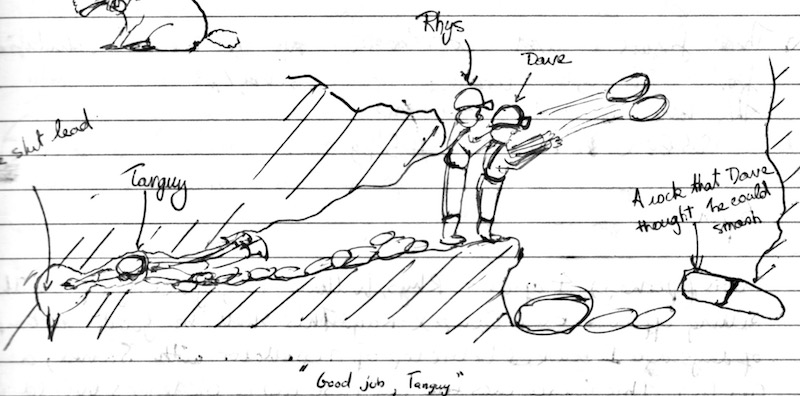
\includegraphics[width=\textwidth]{images/2014/tanguy-jailbreak-2014/migovec_cartoon_14.jpg}}
			\caption{}\label{}
		\end{subfigure}
	\caption{
		\emph{(a)} A plan of Jailbreak cave, drawn in the 2013 scanned logbook --- scanned, from Rhys Tyers 
		\emph{(b)} An artist's impression on digging and subsquently killing the leads in Jailbreak --- scanned, from Tanguy Racine
		}
	
	\end{figure*}

	\bignote{The entrance to the cave was rather tight tube, forcing one to send one arm forward}. The tube emerged into a series of small interconnected chambers, the Barrows, through which I got lost trying to find the way on. The lights and voices of Rhys and Dave below guided me to a fairly unassuming hole in the ground. A thick rope indicated this was the first pitch. I rigged my descender and abseiled to a cunning deviation, where the rope ran through a carabiner directly clipped to the bolt. After this, the pitch slanted at 80 degrees to a boulder choke. Rhys urged me to take care since very little gardening had been done in this cave. Following a fault plane, the passage then dropped into a breakdown chamber where the roof was a largely flat bedding plane. Loose broken limestone blocks lay strewn everywhere on the floor. The chamber was connected to another via a spacious crawl over the cobbles and in a drippy corner we investigated the first lead. This was a small pit, maybe four metres deep, closing down immediately to a small crawl. There, a large boulder (60x60x60cm) blocked the view, and possibly the way on. 

	We decided to use a hauling system. Two of my crabs and my hand-jammer contributed to putting together a pulley jammer while Rhys started to hammer a bolt in the wall above the pit. This involved free climbing directly on top of the drop, and driving the bolt in the rock with only precarious footholds. This was done without any incident, so I climbed down to the rock, wrapped it in slings like a Christmas present and attached them to the rope. Up top, the pulley jammer was put in action, with Rhys attached to the rope, feet against the wall, and Dave adding his weight on the pull. I wedged myself in the pit above the rope, with one hand on the rope. 

	'three? two? one? Heave!' There was a little grunting, a fraction of a second  for the rope to take up all the tension and then a tremor in the boulder which rotated and came swinging vertically below the bolt. Another effort. 'Heave!'. It left the ground, heading towards the rope face and brushed it 'Heave! 'and it was now well off the ground. In no more than five minutes, the rock was almost level with the lip of the drop. In one clean motion, it came to rest on it, with the pulley jammer rope now slack. With three pairs of arms, we managed to move the block away from the drop and shook hands on the success of the operation. 

	Rhys then climbed down, and pronounced the lead dead. Dave turned to me 'Congratulations! You've killed your first lead'. That was a major milestone on the exploration caver's journey. Did the mountain now owe me some fraction of a good find? How many more would I kill before discovering 500m of easy walking passage?

	\begin{figure*}[t!]
	\checkoddpage \ifoddpage \forcerectofloat \else \forceversofloat \fi
		\centering
		\begin{subfigure}[t]{0.517\textwidth}
			\centering
			\frame{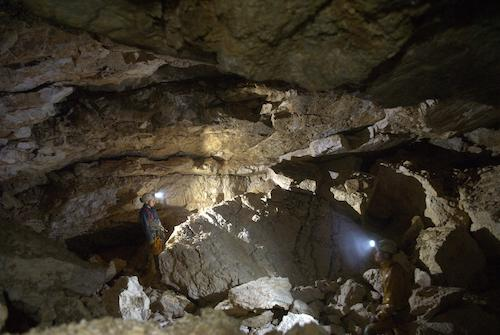
\includegraphics[width=\linewidth]{images/2014/tanguy-jailbreak-2014/rhystyers-jailbreak.jpg}}
			\caption{}
			\label{Inside Jailbreak}
		\end{subfigure}
	\hfill
		\begin{subfigure}[t]{0.463\textwidth}
			\centering
			\frame{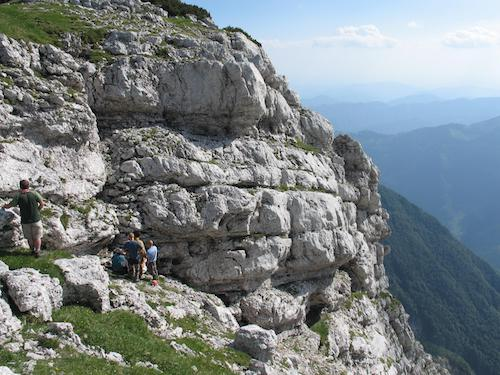
\includegraphics[width=\linewidth]{images/2014/tanguy-jailbreak-2014/petehambley-jailbreak.jpg}}
			\caption{}\label{Entrance to Jailbreak}
		\end{subfigure}
		\caption{ \emph{a} The main chamber at the bottom of Jailbreak (the floor is choked with shattered rock or choss) --- Rhys Tyers \emph{b} The entrance to Jailbreak cave --- Pete Hambley}
	\end{figure*}

	\name{Tanguy Racine}

